El PDM \cite{uddin_post-disaster_2009} originalmente fue planteado como un
modelo de movilidad basado en roles sobre el mapa de la ciudad de
\textit{Helsinki}, Finlandia, para el cual los movimientos de los nodos están
basados en como esa ciudad se organiza luego de un desastre. Por lo tanto, no se
puede aplicar directamente a un país como Chile donde las ciudades tienen rutas
de evacuación y formas de organizarse diferentes a las de otros países.

Por lo tanto se adapta PDM a una ciudad de Chile, en este caso
Valparaíso, utilizando como patrón de movilidad las rutas de evacuación
publicadas por la ONEMI (Oficina Nacional de Emergencia) \cite{evacuacion_valpo}
de Chile. Se elige esta ciudad debido a la información disponible sobre
los lugares de seguridad, el riesgo de \textit{tsunamis} al ser una ciudad
costera con rutas bien definidas de evacuación.

A continuación se describe el proceso de modificación de PDM para adaptarlo al
contexto nacional así como la obtención de un mapa de Valparaíso, utilizando
\textit{osm2wkt} \cite{osm2wkt} compatible con el formato del simulador The ONE.


\seccion{Mejora de \textit{osm2wkt}}

\theone{} \cite{keranen_one_2009} permite definir modelos de movilidad en base a
mapas mediante una clase llamada \textit{MapBasedMovement} ubicada en el
directorio \textit{movement}.  Esta clase utiliza el algoritmo de búsqueda de
camino mínimo sobre el mapa a ser utilizado para encontrar rutas hacia puntos
del escenario.

\figura{Mapa seleccionado de Valparaíso en \textit{Open Street Maps}.}
{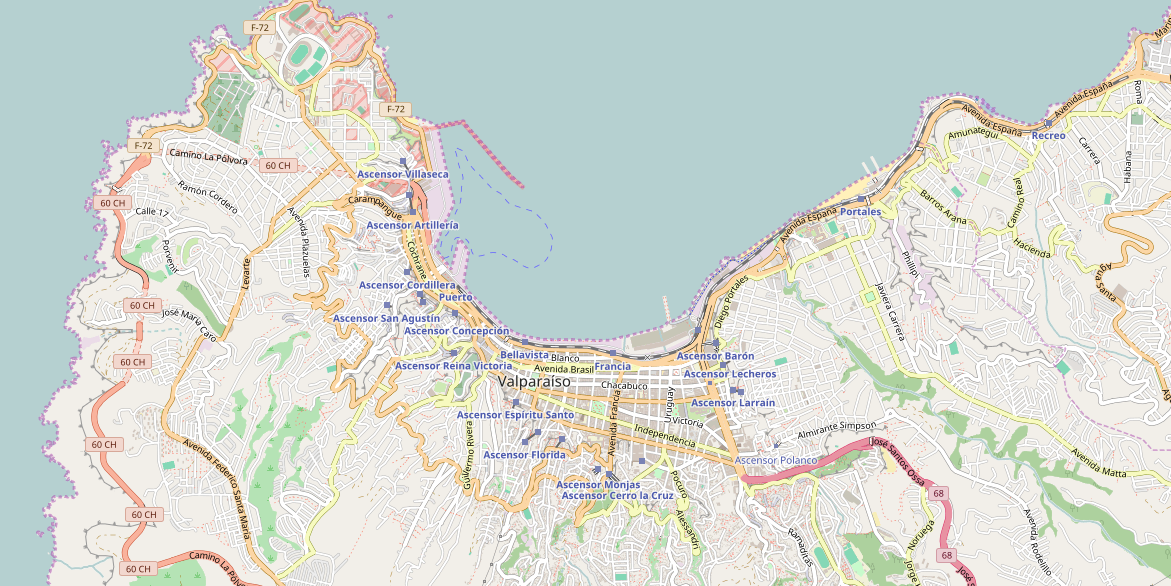
\includegraphics[scale=0.4]{imagenes/valpo/valpo.png}}{fig:valpo-osm}

\figura{Mapa convertido en WKT visualizado en \textit{OpenJump}.}
{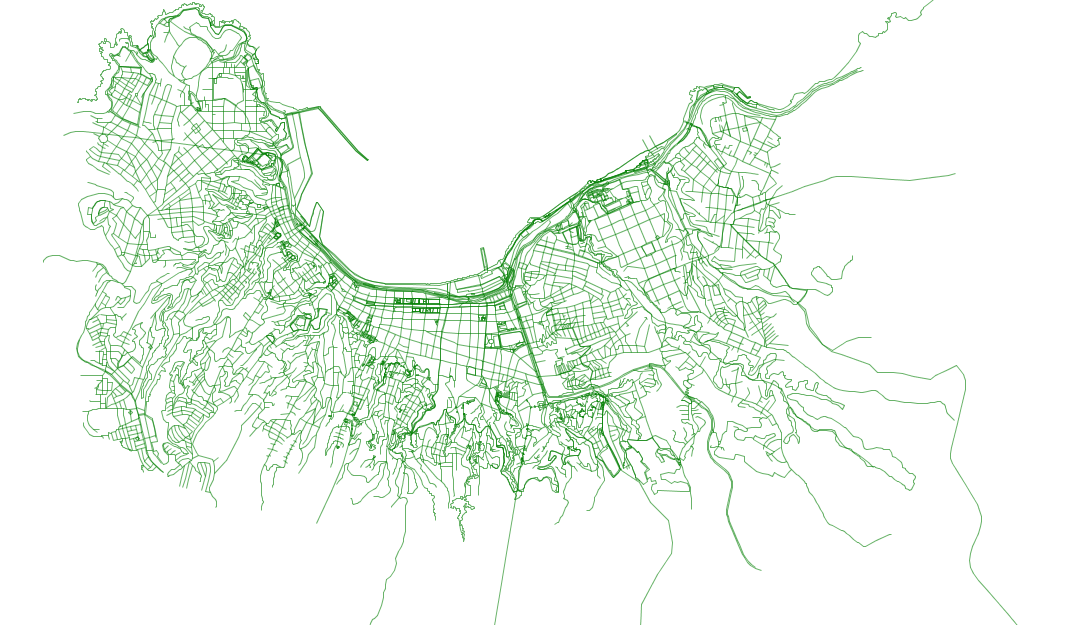
\includegraphics[scale=0.5]{imagenes/valpo/solo_transformado.png}}{fig:valpo-wkt}

El formato de mapa utilizado por \theone{} es WKT (Well Know Text) que define
nodos que componen las rutas que finalmente van a ser las que van a seguir los
nodos. Mediante el programa \textit{osm2wkt} \cite{osm2wkt} se pueden
transformar mapas desde la base de datos de \textit{Open Street Maps} hacia WKT.
En este caso se toma como base la ciudad de Valparaíso como se muestra en la
\ref{fig:valpo-osm}, sector que fue exportado hacia \textit{xml} para ser
utilizado como entrada de \textit{osm2wkt}.  A pesar de lo útil que puede
resultar esta herramienta, no está hecha para transformar ciudades muy grandes
como la de Valparaíso, llevándole un tiempo mayor a una semana en procesar
todas las calles. El tiempo real de procesamiento no se conoce debido a que el
programa se interrumpió su ejecución al alcanzar una semana de procesamiento.

Para tratar de solucionar este problema, se utiliza el \textit{profiler}
\textit{Java Mission Control} \cite{java_mission_control} para encontrar cuales
eran los puntos donde más tiempo está el programa computando. Se identifica
"\textit{fixCompleteness}" como el principal cuello de botella y se procede a
analizar para poder optimizar esa parte del programa. El programa realiza en ese
punto una fase de búsqueda de nodos, que representan los puntos del mapa, para
reparar aquellos nodos que no se encuentren conectados con otros y particiones
del mapa (sectores completamente separados de otros).

El algoritmo implementado en \textit{osm2wkt} tiene una complejidad de
$\mathcal{O}(n^2)$, donde $n$ es el númeor de nodos en el mapa, que a simple
vista no es posible detectar debido a que está implementado como un ciclo simple
con un \textit{while}. La razón de esto es que cada vez que el programa
encuentra un nodo del mapa desconectado, vuelve a revisar todos los nodos
anteriormente revisados para verificar si es que el cambió destruyó algún
arreglo anterior transformando un algoritmo de $\mathcal{O}(n)$ a
$\mathcal{O}(n^2)$ lo hace que el tiempo de procesamiento de los mapas sea de
semanas, trabajo extra que no es necesario debido a que volver a revisar los
nodos pasados una vez se arregla uno no realiza ninguna acción dado que no se
modifican los nodos anteriores. La eliminación de esta sección del código
transforma el algoritmo a $\mathcal{O}(n)$.

Esta mejora logra reducir el tiempo de ejecución del algoritmo permitiendo
obtener un mapa en formato \textit{WKT} en $5.3$ horas.  El mapa convertido es
compatible con \theone{} y no hay problemas de compatibilidad comprobando que no
era necesario verificar nodos anteriores al arreglar el mapa. El mapa final
puede ser observado en la \ref{fig:valpo-wkt} donde cada línea representa un
posible camino que puede tomar el nodo en \theone.


\seccion{Comportamiento e implementación del modelo de movilidad}


A continuación se describen los roles que existen en el modelo de movilidad de
la ciudad de Valparaíso. Los movimientos están basados en los de PDM pero de
igual forma se reimplementan debido a que el código liberado por Uddin et al. no
funciona de la manera en que ellos lo plantean en su publicación de PDM en
\cite{uddin_post-disaster_2009}.


Al igual que PDM, existen 5 tipos de movimientos que reciben el nombre del
código fuente donde fueron implementados:

\begin{itemize}
  \item \textit{AmbulanceMovement}
  \item \textit{CenterMovement}
  \item \textit{CenterToCenter}
  \item \textit{HumanValpoMovement}
  \item \textit{PoliceMovement}
\end{itemize}


Las imágenes utilizadas en esta sección tiene la siguiente nomenclatura: los
círculos naranjos representan a los nodos. Cada nodo tiene un protocolo junto
con todos los requisitos necesarios para ejecutarlo (CPU, RAM, espacio de
almacenamiento, conectividad inalámbrica, etc) mientras que los cuadrados
celestes representan coordenadas o puntos dentro del escenario.


\subseccion{\textit{ValpoConfig}}


\textit{ValpoConfig} contiene toda la información de las posiciones de los
centros que se van a utilizar en el escenario permitiendo a otros nodos
consultar las ubicaciones de centros de suministros o centros de evacuación. Las
posiciones se obtienen leyendo un archivo de texto plano donde cada línea indica
las coordenadas x e y del centro que se esté definiendo. La obtención de las
coordenadas de los centros solamente se realizan para los vecindarios y los
centros de evacuación, el resto de los centros están definidas en el mismo
programa. Estas coordenadas pueden ser revisadas en el \ref{anexo:codigo-valpo}.

Cada una de estas coordenadas es obtenida mediante el programa de visualización
de mapas \textit{OpenJump} \cite{open_jump}, pero hay que tomar en cuenta que
las coordenadas reportadas por este programa no son las mismas que las
utilizadas por \theone, por lo tanto es necesario hacer una transformación
lineal entre las coordenadas para que se correspondan con las del simulador.
Primero se encuentra un punto común de referencia entre ambos programas y se
procede a calcular la diferencia obteniéndose la siguiente ecuación:


\begin{equation}
  x_{one} = x_{oj} - 1239.1806\\
\end{equation}

\begin{equation}
  y_{one} = 2*9586.607714546879 - 4691.8825 - y_{oj}
\end{equation}


Donde $x_{oj}$ e $y_{oj}$ son las coordenadas obtenidas desde \textit{OpenJump}
y $x_{one}$ e $y_{one}$las que se van a utilizar en \theone. La constante
$2*9586.607714546879$ es un ajuste al eje $y$ debido a que este no crece en la
misma dirección del eje de los otros programas. Se realiza una transformación
lineal que se mueva el nodo en la misma dirección en ambos sistemas de coordenada.
Las constantes $1239.1806$ y $4691.8825$ son la diferencia entre el punto
seleccionado como referencia en un programa con el otro. El punto de referencia
seleccionado en \textit{OpenJump} es el $(2633.16858652807, 9585.693473050003)$
mientras que en \theone{} el mismo punto tiene las coordenadas
$(1393.988000,4893.811000)$.

Estas conversiones se realizan para todas las coordenadas en
\textit{ValpoConfig} para no realizarlo manualmente cada vez que se quiera
actualizar la posición de un centro o vecindario.



\subseccion{\textit{AmbulanceMovement}}

Las ambulancias se mueven desde los hospitales hacia puntos aleatorios dentro
del mapa tratando de simular el movimiento desde el centro médico hacia
las distintas emergencias que puedan ocurrir en una ciudad.


\figura{Movimiento de las ambulancias en el modelo de movilidad de Valparaíso.}
{\begin{tikzpicture}

  \begin{scope}[
     xshift=-7.5cm
    ,yshift=-5cm
    ,very thick
    ,node distance=1.6cm
    ,on grid
    ,>=stealth'
    ,block/.style={rectangle,draw,fill=cyan!20}
    ,comp/.style={circle,draw,fill=orange!40}
    ]


  \node [comp] (hospital) [yshift=-3cm] { Hospital };

  \node [block] (evento1) [yshift=-3cm, xshift=-5cm] { Evento aleatorio 1 }
    edge [<-, bend right] node[below] {1}  (hospital)
    edge [->, bend left] node[above] {2} (hospital)
    ;


  \node [block] (evento2) [yshift=-3cm, xshift=5cm] { Evento aleatorio 2 }
    edge [<-, bend right] node[above] {3} (hospital)
    edge [->, bend left] node[below] {4} (hospital)
    ;


  \end{scope}

\end{tikzpicture}
}{fig:mov-ambulancia}


El movimiento se resume en la \ref{fig:mov-ambulancia} donde se puede ver como
una ambulancia va respondiendo a emergencias aleatorias dentro de la ciudad.
Siguiendo el orden de las flechas, primero se mueve desde el hospital hasta el
evento aleatorio 1, para luego volver a su base principal que es el hospital.
Luego repite nuevamente el proceso con el evento aleatorio número 2. Estos
eventos aleatorios no son más que coordenadas generadas aleatoriamente en el
mapa. 

Este movimiento crea conectividad a lo largo de la red al transportar mensajes
entre lugares separados del escenario.


La implementación es una clase Java llamada \textit{AmbulanceMovement} que
hereda de \textit{MapBasedMovement}, utilizando especialmente el método
\textit{getPath} para generar el camino. En general el código consiste en
seleccionar nodos o puntos aleatorios del mapa y luego se vuelve a seleccionar
como llegada el hospital que exista en el escenario. Los caminos se encuentran
utilizando el algoritmo de búsqueda de camino mínimo Dijkstra
\cite{Dijkstra1959} por lo que siempre el nodo sigue la ruta más corta desde la
posición actual al destino. Se utiliza \textit{ValpoConfig} para obtener la
posición del hospital. El hospital fue posicionado en donde se encuentra el
Hospital Carlos van Buren que se encuentra justo fuera de la zona inundable de
la ciudad.


\subseccion{\textit{CenterMovement}}


Este movimiento es el que se le asigna a los nodos que van a actuar como
centros. Simplemente le asigna una coordenada inicial al nodo y en los
siguientes pasos de la simulación lo deja quieto. Las coordenadas de
las posiciones de los centros son de \textit{ValpoConfig}. Los centros fueron
colocados de manera uniforme fuera de la zona inundable, a excepción de la zona
segura para el cual se utilizaron planes de evacuación de la ONEMI.


\subseccion{\textit{CenterToCenter}}


El movimiento de los vehículos de suministros esta dictado por este tipo de
movilidad que consiste en la selección de un centro de suministro aleatorio como
destino. Cada vez que se llega al destino, que es un centro, se vuelve a
seleccionar otro de los disponibles que existen en el escenario.


\figura{Dos posibles movimientos entre centros de suministros en el modelo de movilidad
de Valparaíso, uno marcado con línea continua y otro punteada.}
{\begin{tikzpicture}

  \begin{scope}[
     xshift=-7.5cm
    ,yshift=-5cm
    ,very thick
    ,node distance=1.6cm
    ,on grid
    ,>=stealth'
    ,block/.style={rectangle,draw,fill=cyan!20}
    ,comp/.style={circle,draw,fill=orange!40}
    ]


  \node [comp] (centro1) [xshift=-3cm] { Centro de suministros 1 };
  \node [comp] (centro2) [xshift=3cm] { Centro de suministros 2 }
    edge [<-]  node[above] {1} (centro1) 
    ;
  \node [comp] (centro3) [yshift=-5cm] { Centro de suministros 3 }
    edge [<-, bend left] node[right] {1} (centro2)
    edge [<-, dashed] node[left] {2} (centro1)
    edge [->, bend right, dashed] node[right] {2} (centro2)
    ;


  %\node [comp] (hospital) [yshift=-3cm] { Hospital };

  %\node [block] (evento1) [yshift=-3cm, xshift=-5cm] { Evento aleatorio 1 }
    %edge [<-, bend right] (hospital)
    %edge [->, bend left] (hospital)
    %;


  %\node [block] (evento2) [yshift=-3cm, xshift=5cm] { Evento aleatorio 2 }
    %edge [<-, bend right] (hospital)
    %edge [->, bend left] (hospital)
    %;


  \end{scope}

\end{tikzpicture}
}{fig:movimiento-centro-centro}

El movimiento se puede ver en la \ref{fig:movimiento-centro-centro} donde se
representan dos movimientos posibles, ambos comenzando en el centro de
suministros 1. El primer movimiento decide moverse al centro 2 y luego al 3
(línea continua) y el segundo se mueve primero hacia el centro 3 y luego al 2
(línea punteada).

La configuración general del modelo de movilidad se encuentra en una clase Java
llamada \textit{CenterToCenter} donde el método \textit{getPath} es el encargado
de entregar un camino a seguir hacia el centro seleccionado aleatoriamente. Las
posiciones de los centros de suministros se obtienen utilizando métodos de la
clase \textit{ValpoConfig}.

En total se definieron 11 centros de evacuación o zonas seguras, 5 centros de
suministros y un centro de coordinación de rescate fuera de la zona inundable.
Dentro de la zona inundable se definieron 11 vecindarios por los cuales las
personas se mueven antes de la alarma de evacuación y después que se levanta la
alerta. Las coordenadas específicas, definidas en \textit{OpenJump}, pueden ser
vistas en el \ref{anexo:codigo-valpo}.


\subseccion{\textit{HumanValpoMovement}}

Este es el movimiento más complejo del modelo debido a que trata de recrear el
comportamiento que realizan las personas durante una evacuación en una ciudad
como Valparaíso. El contexto en el cual se desenvuelve es evacuaciones de las
zonas inundables de la ciudad en caso de alerta de \textit{tsunami} luego de un
terremoto en alguna parte del pacífico, especialmente en el mismo país.

Inicialmente, las personas se encuentran en sus vecindarios recorriendo las calles
de manera aleatoria asumiendo que esta primera etapa ocurre luego de un evento
como un terremoto en el país. Luego de una cantidad de tiempo ajustable, se
espera que las autoridades como el SHOA (Servicio Hidrográfico y Oceanográfico
de la Armada) den la orden de evacuación de la zona inundable por lo tanto las
personas deberían moverse de sus hogares a los lugares seguros definidos
previamente por la ONEMI (Oficina Nacional de Emergencias). Una vez llegan al
lugar definido como seguro, las personas esperan a que se levante la orden de
evacuación para volver a sus hogares. Al volver a sus hogares las personas
vuelven al estado anterior de moverse en el vecindario para asegurarse que todo
se encuentre en orden.


De acuerdo al Manual de Operaciones del Centro de Alerta Temprana (C.A.T.)
\cite{manual_cat} de la ONEMI, existe un tiempo máximo de 5 minutos luego de un
evento para crear los primeros informes, por lo tanto las personas deberían
comenzar evacuar la zona inundable desde entre los 5 a 10 minutos iniciada la
simulación, asumiendo que esta comienza al final el sismo. El margen de tiempo
de evacuación está dada por una distribución de Pareto que es la utilizada en el
modelo de movilidad PDM para el caso de los tiempos de retorno en
\textit{Helsinki}.

Los refugios o zonas seguras deben poder contener a la población por al menos
$12$ horas luego de ocurrido el evento \cite{guia_referencia_onemi}, por lo
tanto se va a utilizar este tiempo como el de permanencia en la zona segura, que
es equivalente a $43200$ segundos de simulación.


\figura{Diagrama de transición para el movimiento de las personas en Valparaíso.}
{\begin{tikzpicture} 

  \umlstateinitial[name=init, x=-11, y=0.25]{Inicial}
  \umlbasicstate[name=mov, x=-6]{Movimiento Vecindario}
  \umlbasicstate[name=evacuacion, x=2]{Evacuación}
  \umlbasicstate[name=espera, x=2, y=-4]{Espera}
  \umlbasicstate[name=retorno, x=-6, y=-4]{Retorno}

  \umltrans[arg=Terremoto, pos=0.5]{init}{mov} 
  \umltrans[arg=Alarma de evacuación, pos=0.5]{mov}{evacuacion} 
  \umltrans[arg=Llegada a lugar seguro, pos=0.5]{evacuacion}{espera}
  \umltrans[arg=Se levanta alarma, pos=0.5]{espera}{retorno}
  \umltrans[arg=Llegada al vecindario, pos=0.5]{retorno}{mov}

\end{tikzpicture}
}{fig:personas-transisicion}

Este modelo de movilidad puede ser explicado en un diagrama de transición donde
existen 4 estados: movimiento en vecindario, evacuación, espera retorno y
retorno, como se puede ver en la \ref{fig:personas-transisicion}.

La fase de evacuación continua hasta que se llega a un centro de evacuación,
utilizando la nomenclatura de PDM, o zona segura. El recorrido de la ruta a
seguir se obtiene del documento de evacuación proporcionado por la ONEMI de la
\ref{fig:valpo-evacuacion}.


\figuraFuente{Rutas propuestas por la ONEMI para evacuar la zona inundable de Valparaíso.}
{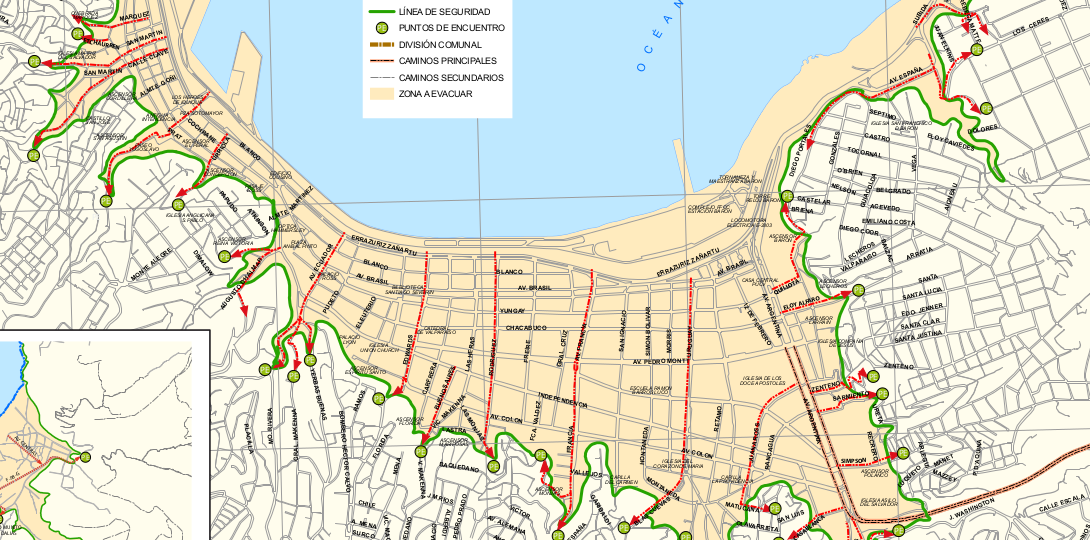
\includegraphics[scale=0.4]{imagenes/valpo/evacuacion.png}}{fig:valpo-evacuacion}
{Dirección regional de ONEMI, Valparaíso, (2016)}

Estas rutas fueron modeladas tomando solamente las que se encuentran cerca de la
bahía principal. Utilizando nuevamente \textit{OpenJump} para visualizar el mapa
se crearon los puntos que deben seguir las personas para llegar a su zona de
seguridad más cercana.


\figura{Puntos a seguir por lo nodos hacia las zona de seguridad.}
{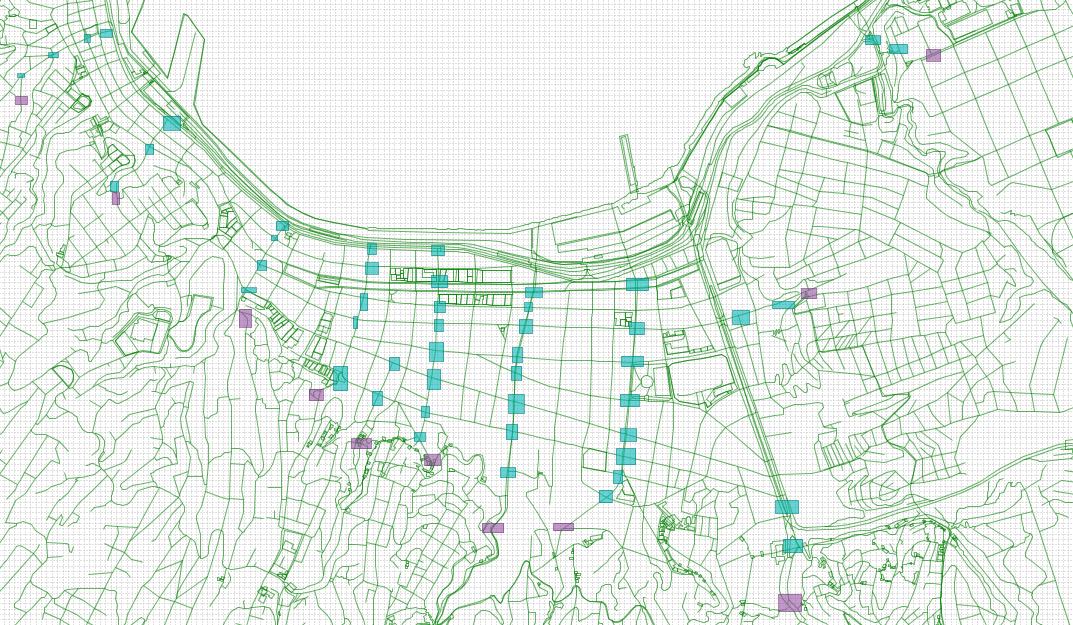
\includegraphics[scale=0.4]{imagenes/valpo/waypoints.png}}{fig:valpo-evacuacion-way}


En la \ref{fig:valpo-evacuacion-way} se muestran los caminos a seguir marcados con
cuadrados azules y las respectivas zonas seguras como cuadrados morados. Cuando
se da la alerta de evacuar cada persona busca la sección de camino a evacuar más
cercano y se dirige hacia el mediante el camino mínimo entregado por el algoritmo de
Dijkstra. Una vez se llega a la sección del camino más cercano, se comienza a
avanzar hacia la zona de seguridad siguiendo los puntos del camino. Cuando se
llega a la zona de seguridad se termina de avanzar y se espera a la orden de
evacuar.

El camino de vuelta consiste en moverse nuevamente al vecindario donde se
encontraba originalmente la persona para luego continuar con el movimiento
original.




\subseccion{\textit{PoliceMovement}}

La policía, en la notación de PDM, o carabineros son vehículos que se mueven por
la ciudad desde un centro de policía hacia los vecindarios verificando que todo
se encuentre en orden. En este movimiento se localizaron las comisarías fuera de
la zona inundable de la ciudad mediante \textit{Google Maps} como base para 
$10$ patrullas. Las patrullas realizan un movimiento que comienza en la comisaría y va hacia
los vecindarios y zonas seguras creando conectividad en la red entre las
particiones que se encuentran desconectadas.




\figura{Movimiento de las patrullas en el modelo de movilidad de Valparaíso.}
{\begin{tikzpicture}

  \begin{scope}[
     xshift=-7.5cm
    ,yshift=-5cm
    ,very thick
    ,node distance=1.6cm
    ,on grid
    ,>=stealth'
    ,block/.style={rectangle,draw,fill=cyan!20}
    ,comp/.style={circle,draw,fill=orange!40}
    ]


  \node [comp] (comisaria) [yshift=-3cm] { Comisaría };

  \node [block] (evento1) [yshift=-3cm, xshift=-5cm] { Vecindario aleatorio 1 }
    edge [<-, bend right] node[below] {1} (comisaria)
    edge [->, bend left] node[above] {2}  (comisaria)
    ;


  \node [block] (evento2) [yshift=-3cm, xshift=5cm] { Vecindario aleatorio 2 }
    edge [<-, bend right] node[above] {3} (comisaria)
    edge [->, bend left] node[below] {4}  (comisaria)
    ;


  \end{scope}

\end{tikzpicture}
}{fig:mov-patrulla}


El movimiento puede ser visto en la \ref{fig:mov-patrulla} y si se compara con
el movimiento que realizan las ambulancias, se puede notar que es muy similar,
con la diferencia que en vez de ser puntos aleatorios del mapa son vecindarios
aleatorios. La patrulla selecciona un vecindario a visitar donde realiza un
movimiento aleatorio verificando que todo esté en orden dentro de él. Luego que
el tiempo establecido se cumple, se retorna a la comisaría de origen, la cual
actúa como hogar de la patrulla.


\subseccion{Velocidades de movimiento}

Para una estimación de la velocidad de movimiento de las personas, se utiliza la
Guía de referencia para sistemas comunales de evacuación por \textit{tsunami}
\cite{guia_referencia_onemi}. Esta presenta una tabla donde se puede establecer la
relación entre el grado de pendiente y la velocidad de desplazamiento a las
zonas seguras de evacuación. El grado de la pendiente puede ser obtenido de la
Carta de inundación por \textit{tsunami} de Valparaíso-Viña del Mar
\cite{curvas_nivel} publicada por el SHOA donde se encuentran las curvas de nivel
para la ciudad de Valparaíso. Las personas que se muevan desde las zonas en
riesgo a las zonas seguras experimentan un cambio de altura de 10 metros de
acuerdo a ese documento. Con \textit{Google Maps} se puede obtener que la
distancia del centro a la zona segura más cercana es $300$ metros y por lo tanto
se puede obtener el ángulo de la pendiente la ecuación (\ref{eq:pendiente})
resultando en la ecuación (\ref{eq:pendiente_resultado}).

\begin{equation}
  \tan \theta = \frac{altura}{distancia}
  \label{eq:pendiente}
\end{equation}


\begin{equation}
  \theta = \tan^{-1}(\frac{10}{300}) = 1,9 \degree
  \label{eq:pendiente_resultado}
\end{equation}

Finalmente, de acuerdo a la tabla de la ONEMI, las personas deberían moverse a
una velocidad de $4,48$ km/h o $2,244$ m/s en promedio.

La velocidad de los vehículos fue asignada a $8.3$ m/s o $30$ k/h, la cual es la
mitad de la velocidad máxima permitida en Chile de $60$ k/h \cite{velocidad}.


\seccion{Evaluación del modelo de movilidad}
\customlabel{sec:evaluacion-movilidad}{Subcapítulo \arabic{chapter}.\arabic{section}}


El modelo de movilidad propuesto fue evaluado utilizando las métricas de Nelson
et al. \cite{Nelson2007} donde se le da una gran importancia a las relacionadas
con la densidad de los nodos debido a que estas métricas permite evaluar que tan
desafiante es un modelo de movilidad para los protocolos DTN ya que, al obtener
una baja densidad de nodos se puede decir que la red está altamente
particionada. Las métricas utilizadas son las siguientes:

\begin{itemize}
  \item Coeficiente de \textit{clustering}: Mide que tan conectados están los
    vecinos de un nodo en particular y se calcula localmente. Un valor alto
    indica que la red tiende a formar \textit{clusters} de nodos.
  \item Promedio de la densidad de nodos en el tiempo: Muestra como la densidad
    de nodos cambia en el tiempo. Esto es especialmente importante en un
    escenario como el propuesto debido a que los movimientos de los nodos
    cambian ante los eventos de evacuación alterando la densidad.
  \item Densidad máxima en el tiempo: Entrega información sobre los tamaños de
    los \textit{clusters} creados en el modelo, siendo esta una heurística más
    barata de calcular que los tamaños reales de los \textit{clusters}, que
    implicaría el uso de algoritmos de grafos.
  \item Varianza de la densidad de nodos en el tiempo: Entrega información sobre
    la varianza de los tamaños de los \textit{clusters} en el tiempo, lo que
    puede indicar que tan diferentes son algunas partes de la red.
\end{itemize}

Para implementar estas métricas se considera que dos nodos son vecinos cuando
existe una conexión inalámbrica entre ellos por medio de la interfaz
\textit{Bluetooth} que tiene un rango de $100$ metros. Las configuraciones del
modelo de movilidad de Valparaíso consisten en las ya explicadas en este
capítulo.


Se ejecutaron simulaciones del nuevo modelo de movilidad de Valparaíso o
Valparaíso Mobility Model (VMM), \textit{Post-Disaster Mobility Model} (PDM) y
\textit{Working Day Mobility Model} (WDMM), para ver cual es el comportamiento y
que tan desafiantes son los modelos para un protocolo DTN.

Las configuraciones de PDM consisten en: 10 vecindarios, 2 centro
de coordinación, 5 refugios, 1 centro de policía, 1 hospital, 5 vehículos de
suministros, 20 rescatistas y 200 personas.

El modelo de movilidad WDMM utiliza la configuración indicada en la publicación
que lo define que consiste en 2 buses y 150 personas.




%\pgfplotsset{cycle list/Dark2}
%\pgfplotsset{cycle list/Set1}
\pgfplotsset{cycle list/Set2}
\newcommand{\colorscheme}{Set2}


% Argumentos
% 1: Archivo entrada
% 2: Titulo
% 3: Label x
% 4: Label y
\newcommand{\graficoprotocolos}[4]{
\begin{tikzpicture}
\begin{axis}[
    xlabel={#3},
    ylabel={#4},
    title=#2,
    grid=major,
    legend entries = {Epidemic, MaxProp},
    legend style = {
      legend pos = outer north east,
    },
    mark = *,
    cycle multi list=\colorscheme
  ]
\pgfplotstableread{#1}\mydata;
\addplot table [] {\mydata};
\end{axis}
\end{tikzpicture}
}


En la \ref{fig:coeficiente-comparacion} se pueden ver los resultados del
coeficiente de \textit{clustering} de los distintos modelos de movilidad
evaluados. Se puede ver que en un principio PDM tiende a formar una cantidad un
poco más alta de \textit{clusters} que los otros dos modelos de movilidad,
indicando que en PDM, cuando las personas se encuentran en los refugios, en
promedio tienden a crear menos \textit{clusters}. Por otro lado, los tres modelos a
partir de los $15000$ segundos de simulación ocurre un cambio provocado por
eventos dentro de la simulación, en el caso de PDM y VMM volver a los
hogares y en el caso de WDMM ir a trabajar. Este cambio provoca que los nodos
ahora formen una mayor cantidad de \textit{clusters} haciendo más fácil el
transporte de mensajes debido a que existe una mayor cantidad de conexiones.
PDM y Valparaíso mantienen un coeficiente relativamente alto por el resto de la
simulación mientras que WDMM vuelve a bajar cuando las personas vuelven a sus
hogares. En el \ref{anexo:wdmm-movilidad} se puede ver el ciclo completo de WDMM
para varios días de simulación.


\figura{Comparación del coeficiente de \textit{clustering} en el tiempo.}{
\graficoMovilidad{Coeficiente de \textit{clusterting}}
{data/movilidad/pdm_clustering.txt}
{data/movilidad/wdmm_clustering.txt}
{data/movilidad/valpo_clustering.txt}}
{fig:coeficiente-comparacion}


La densidad promedio de los nodos en la red puede ser observada en
\ref{fig:promedio-densidad-comparacion} donde se ve que PDM tiene una mayor
concentración de nodos, alcanzando un promedio de $45$ nodos entre 0 y $20000$
segundos de simulación mientras que VMM alcanza $20$ nodos promedio. La
diferencia entre ambos se debe a la cantidad de refugios disponibles entre ambos
modelos: PDM tiene un total de $5$ centros de evacuación mientras que VMM
tiene un total de $10$ zonas seguras definidas, es decir, el doble. Esto explica
porque la cantidad promedio de nodos es la mitad en VMM que en PDM y, por
lo tanto, PDM tiende a generar \textit{clusters} más grandes en promedio que el
modelo de VMM. 

Por el lado de WDMM, existe una densidad menor a lo largo de toda la simulación
lo que muestra que el movimiento definido en este modelo presenta un desafío
distinto a los otros modelos de movilidad: en vez de tener un problema de
consumo de energía relacionado con la copia de mensajes como en PDM y VMM que
surge de su alta densidad, presenta un problema de baja tasa de entrega debido a
su baja densidad de nodos. Finalmente, PDM y VMM no tienen una diferencia
significativa en el resto de la simulación una vez las evacuaciones terminan y
las personas retornan a sus hogares.


\figura{Comparación del promedio de densidad de nodos en el tiempo.}{
\graficoMovilidad{Cantidad de nodos vecinos (promedio)}
{data/movilidad/pdm_densidad.txt}
{data/movilidad/wdmm_densidad.txt}
{data/movilidad/valpo_densidad.txt}}
{fig:promedio-densidad-comparacion}


La \ref{fig:maximo-densidad-comparacion} muestra la densidad máxima de los
\textit{clusters} formados en el tiempo. Se puede ver que el \textit{cluster} de
mayor tamaño es creado en PDM mientras que en VMM se llega a un cluster
de tamaño máximo de $50$. Esta métrica indica que el modelo de movilidad PDM
tiende a ser menos exigente para los protocolos DTN, en los primeros momentos de
la simulación, debido a que los nodos tienden a formar clusters más grandes que
los otros modelos de movilidad. WDMM tiene cambios de métricas mucho menores que
el resto de los modelos de movilidad lo que indica que no existen cambios
importantes en la movilidad de los nodos, al menos cuando se compara con PDM y
VMM, pero sigue presentando el desafío de la baja densidad de nodos que puede
causar una baja tasa de entrega en la red.



\figura{Comparación del máximo de la densidad de nodos en el tiempo.}{
\graficoMovilidad{Cantidad de nodos vecinos (máximo)}
{data/movilidad/pdm_densidad_maxima.txt}
{data/movilidad/wdmm_densidad_maxima.txt}
{data/movilidad/valpo_densidad_maxima.txt}}
{fig:maximo-densidad-comparacion}


Finalmente, la varianza de la densidad de nodos puede ser vista en
\ref{fig:varianza-densidad-comparacion}. Esto indica que tan diferentes son los
tamaños de los \textit{clusters} creados en cada modelo de movilidad. Se puede
ver que PDM es quien genera los \textit{clusters} más desiguales de todos los
modelos de movilidad indicando que es un buen candidato para probar protocolos
que sean adaptativos, debido a las diferencias de conectividad entre los nodos.
Esta diferencia entre PDM y VMM se puede explicar por la cantidad
desigual de personas que llegan a un refugio o zona segura.

Por otro lado, WDMM es homogéneo respecto a los otros modelos de movilidad por
lo tanto existen menos diferencias signifcativas entre nodos de la red.


\figura{Comparación de la varianza de la densidad de nodos en el tiempo.}{
\graficoMovilidad{Cantidad al cuadrado de nodos vecinos (varianza)}
{data/movilidad/pdm_varianza.txt}
{data/movilidad/wdmm_varianza.txt}
{data/movilidad/valpo_varianza.txt}}
{fig:varianza-densidad-comparacion}


\seccion{Conclusiones del modelo de movilidad}

El modelo de movilidad basado en Valparaíso (VMM) permite probar los protocolos en un
ambiente más parecido al chileno que la ciudad original planteada en PDM
(Helsinki), dentro de las limitaciones de tiempo y capacidad de computo del
simulador \theone. En el estado del arte no se encontraron modelos de movilidad
basados en planes de evacuación chilenos, por lo que esta adaptación de
PDM es un aporte nuevo a la investigación de redes en desastres naturales en
Chile.

En el contexto de esta tesis este modelo de movilidad se plantea como otra forma
más de evaluar el comportamiento del protocolo creado.

Al comparar el modelo de movilidad nuevo con PDM, se puede ver que el comportamiento es
similar: existe un momento de evacuación, un momento de espera y un momento de
retorno al los hogares, pero la diferencia principal surge de las ciudades
utilizadas y de la forma de organizarse ante un desastre, lo que muestra que
existe una diferencia entre Helsinki y Valparaíso o entre un escenario de
desastre nacional y uno extranjero.

Como trabajo futuro en está área se debe trabajar en hacer más realista el
modelo de movilidad modificando en mayor medida los movimiento de los
rescatistas y vehículos de emergencia de acuerdo a los protocolos establecidos
en Chile.

